\section{Literature Review}
\begin{figure}[h]
    \centering
    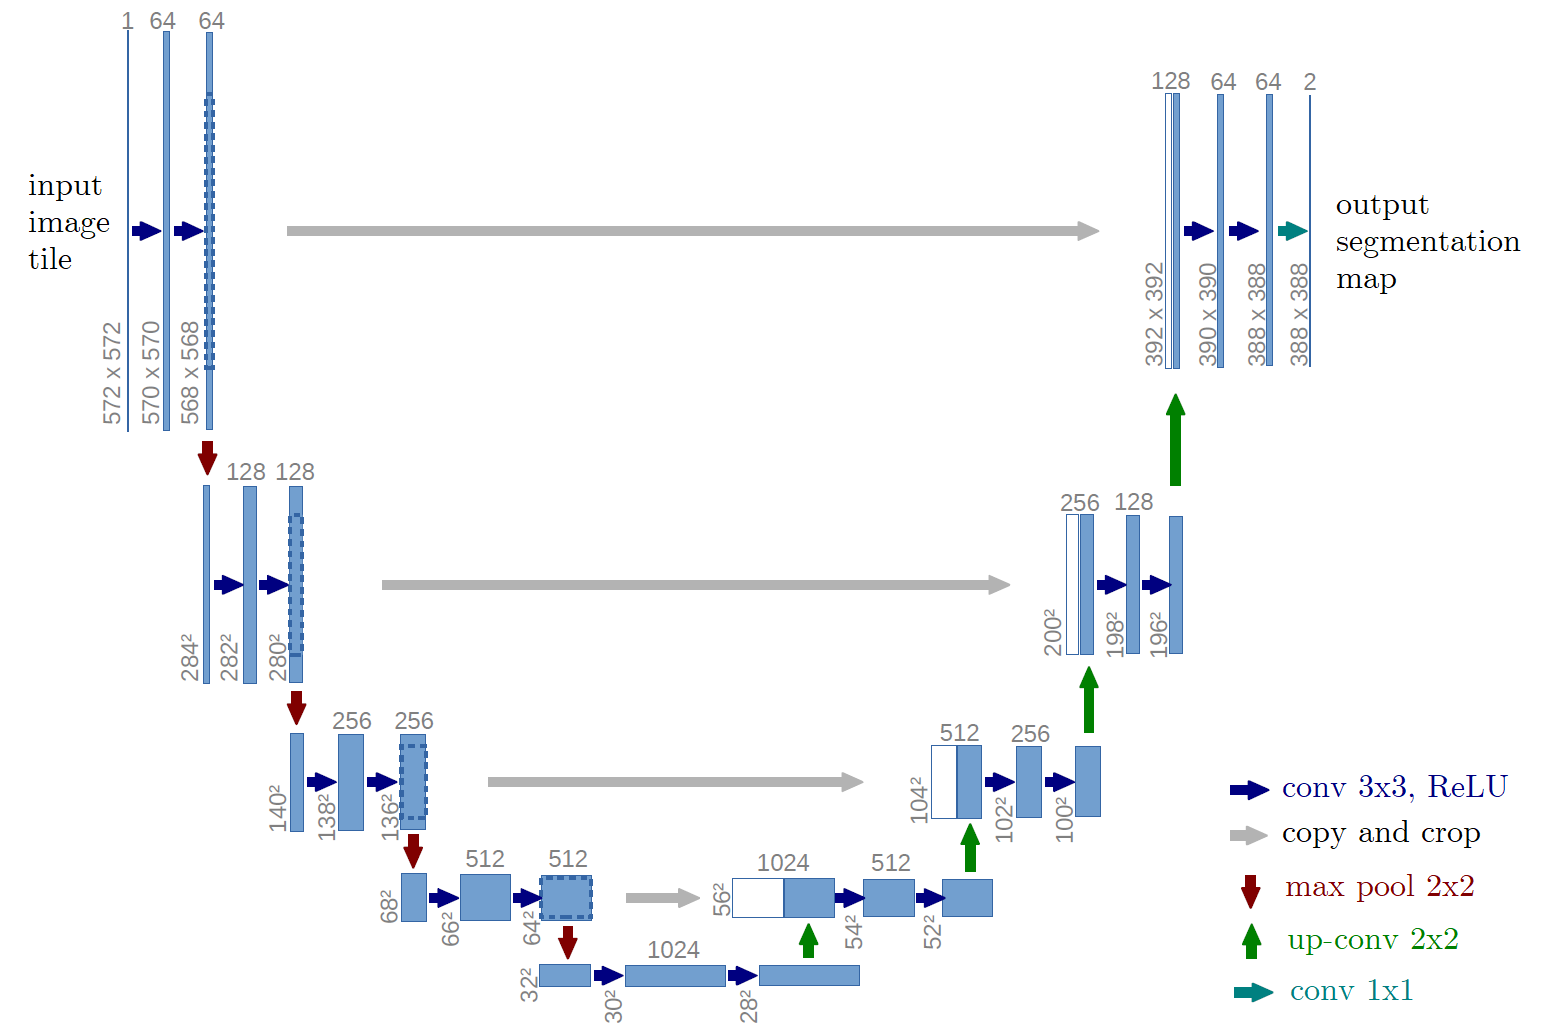
\includegraphics[width=0.9\textwidth]{images/u-net-architecture}
    \caption{U-Net Architecture \cite{unet15}}
    \label{fig:unet_architecture}
\end{figure}

\subsection{Convolution}
\cite{DLbook16}
326: convolutional neural networks (CNN) are specialized kind of neural network for data with grid-like topology, for example images as 2D pixel grid. CNN are basically NN that use at least one convolutional layer.

330: NN use only matrix multiplication. meaning every output unit of one layer interacts with the all input units of the next layer. convolution leverages sparse interactions. for example images can have millions of pixels, but to detect edges it is enough to only look at a few pixels at a time. thus we can have a kernel smaller than the image size resulting in fewer parameters. This reduces memory requirements of the model and increases statistical efficiency.

331, 333: another advantage is parameter sharing. with matrix multiplication you usually have a weight matrix, where each value is used only once. convolution operation uses parameter sharing, because one kernel is applied multiple times on the same image. and since kernel is smaller than image, it again reduces number of parameters by a significant amount.

334f: due to parameter sharing, convolution operation is equivariant to translation. Meaning, if you move parts of the input convolution will still give you the same output, just with the moved detection. This is especially helpful for working with images, as object might be in different locations of the image, but should still be realized.

\subsection{Pooling}
\cite{DLbook16}
335: Pooling replaces output of certain location with a summary of the nearby outputs. Max Pooling reports the maximum value inside a rectangular neighborhood. Other functions: (weighted) average or $L^2$ norm.


\begin{figure}[h]
    \centering
    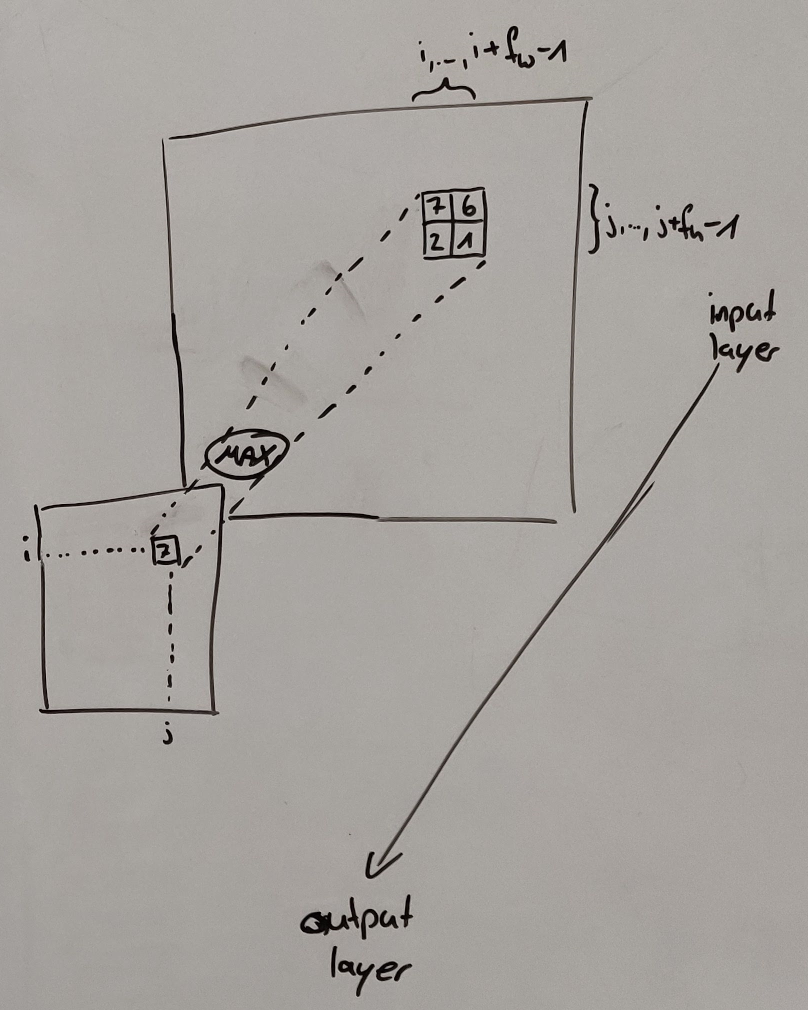
\includegraphics[width=0.8\textwidth]{images/maxpool}
    \caption{Max pooling \cite{stanford_convnet}}
    \label{fig:pooling}
\end{figure}

\cite{stanford_convnet}
Module 2: pooling layers between conv layers are common architecture. thereby you progressively reduce the spatial size and also number of params later in the net. pooling operates on all feature maps independently. For example pooling with kernel size 2x2 and stride 2 downsamples the input, so that 75\% of information is discarded.

Pooling layer are not trainable, because they compute a given function on the input elements. This function is oftentimes MAX function, also other variation like AVG oder L2-norm are used. However, pooling is configurable for the hyperparameters kernel size and stride.

\subsection{U-Net architecture}
\cite{unet15}
network architecture consists of a contracting path and an expansive path. contraction follows the typical architecture of convolutional network. repeated application of 3x3 convolutions, followed by ReLU and 2x2 max pooling. stride 2 for downsampling, features double for each contraction.
expansive path is upsampling followed by 2x2 convolution. also concatenation of the cropped feature map from the corresponding feature map from contraction path.
final layer is 1x1 convolution to map feature vector to desired number of classes. Demonstrated results with the EM segmentation challenge (\cite{isbi_challenge}), where they achieved very good results.


\newpage